Voxie supports the display of raw images. A raw image is a single projection from the ct.
Its visual representation is defined by its pixel values.

Voxie supports multiple operations on raw images. This includes adjusting, colorizing, analyzing.

\subsubsection{Creating a raw visualizer}

A raw visualizer is created by opening a file which contains raw images. In the UI this is done by right clicking in the object tree and pressing on \textit{Open File} and select the file.
After loading the file, click right on it in the object tree and press create \textit{Create Rawvisualizer}. 

\subsubsection{The raw image view}

By default the raw image view window offers a canvas that displays the raw associated with the raw image view. It also allows for tools to be used which can modify the slice or display information. Tools can be switched by using the number keys.

\subsubsection{Zoom / Move Tool}

The zoom and move tool allows one to zoom and move around the displayed image. Holding the left mouse button and dragging will move the image around. The mouse wheel is used to zoom the image. Toggling the checkbox labeled \textit{Drag redraw?} will allow for less processing power to be required as the image will only be altered when the mouse button is released.

\subsubsection{Slice View Sections}

A slice view creates six new sections on initialization.

\begin{itemize}
  \item{\emph{Select Picture\newline The select picture section allows to select a new picture by its number and shows it after it has been loaded.}}
  \item{\emph{Colorizer}\newline The colorizer section maps values to colors. In between values will be interpolated.}
  \item{\emph{Histogram}\newline The value distribution is visualized here. It also offers advanced options like logarithmic scaling.}
  \item{\emph{Options menu}\newline The menu includes two sliders which can adjust the rate of the slide show speed and the amount of buffered raw images. There is also a button to stop all queue loading operations for this dataset. For the change of the buffer size to go in effect the apply button needs to be pressed. Warning: Changing the buffers size may affect your performance depending on your computer specifications.}
\end{itemize}

\subsubsection{Colorizer}

The colorizer maps values to colors. Colors in between the given mappings will be interpolated. A color mapping can be added by pressing the \emph{Add Mapping} button in the first column. This will add a new mapping to the list of mappings below.\newline The colors can be changed by clicking on the displayed color. This will invoke the operating system specific color picker. \newline To remove a mapping simply click on the \emph{Remove Mapping} button. \newline Please note that mappings with the same value will be automatically merged, the new mapping having priority. \newline A click on the gear button opens a small options menu with two options: \emph{Calculate Mapping} automatically calculates a color mapping of two values by using an algorithm based on the whole 3D dataset. \emph{Default mapping} removes the color mapping and replaces it with the default one (0 = black, 1 = white).

\begin{figure}[h!]
  \centering
  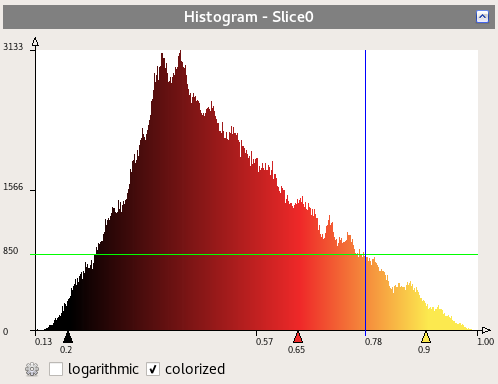
\includegraphics[scale=0.5]{img/2d/histogram}
  \caption{Histogram Section}
\end{figure}  

\subsubsection{Histogram}

The histogram section shows a visualization of the value distribution of the slice. The scale can be set to linear or logarithmic by switching the \emph{logarithmic} check box. 
\newline The histogram can be colorized dependant on the color mapping values by activating the \emph{colorized} check box. The color mapping (adjusted in the Colorizer) is also permanently shown along the X-Axis as colored triangles.\newline Points within the histogram widget can be marked by a left click with the mouse in the desired area. Move the marker by holding the left mouse button. The related values are shown down the x and y axis. Deleting a marked point works by right clicking with the mouse inside the histogram widget.\newline A gear symbol opens the options dialog. By default, the bouds of the axes are calculated automatically in a way that all values are displayed within the histogram widget. Manual bounds are possible by deactivating the \emph{automatic} checkboxes and setting specific values in the related text boxes. \newline The non-colorized histogram is red by default without a background color. Those color values are adjustable manually by clicking on the colored boxes. \newline The histogram widget can be adjusted in height. This is useful for accurate work.\newline \emph{Hint: All values are applied in real time. Watch the histogram while adjusting the values to get better results}.

\begin{figure}[h!]
  \centering
  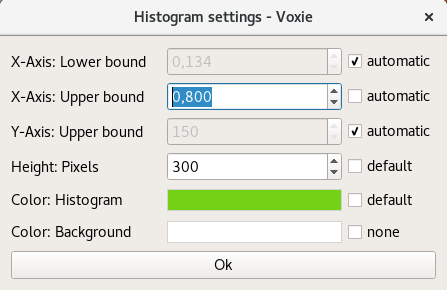
\includegraphics[scale=0.5]{img/2d/histosettings}
  \caption{Histogram Options}
\end{figure}  

\subsubsection{Change image toolbar}

The toolbar is attached below the raw image view and consists of three buttons

\begin{itemize}
\item Forwards button
\item Backwards button
\item Start/Stop slide show button 
\end{itemize}

The forwards/backwards button both move through the pictures in the respective direction. The visualizer also stores how many times you pressed a button, meaning if you press 10x the forward button the visualizer will show as soon as the pictures are available, the next 10 picture originating from your current picture.
The start/stop button starts or stops the slide show which loops through the entire raw dataset. If too many loading commands were executed, it is possible to clear them all out by pressing the \textit{Clear Queue} button in the options menu in the sidebar.
